\section{Quantum Mechanics Foundations}
\label{sec:quantum-foundations}

This section establishes the quantum mechanical principles that underpin quantum automata theory. We emphasise both the mathematical formalism and the conceptual distinctions from classical systems. In what follows, we review the basic postulates of quantum mechanics, elaborate on the structure and evolution of quantum states, and discuss measurement, decoherence, and their computational implications.



\subsection{Qubits and Quantum States}
\label{subsec:qubits}

\begin{definition}[Qubit]
A \emph{\gls{qubit}} is the fundamental unit of quantum information. It is represented as a normalised vector in a two-dimensional complex Hilbert space,
\[
\mathcal{H} = \mathbb{C}^2.
\]
\end{definition}

\begin{notation}[Computational Basis]
The standard (computational) basis states for a qubit are defined as
\[
|0\rangle = \begin{pmatrix} 1 \\ 0 \end{pmatrix}, \quad |1\rangle = \begin{pmatrix} 0 \\ 1 \end{pmatrix}.
\]
\end{notation}

\begin{definition}[General Qubit State]
A general state of a \gls{qubit} is given by
\[
|\psi\rangle = \alpha|0\rangle + \beta|1\rangle, \quad \text{with } |\alpha|^2 + |\beta|^2 = 1,
\]
where \(\alpha,\beta \in \mathbb{C}\) are the \emph{probability amplitudes}.
\end{definition}

\begin{remark}
Global phase factors—i.e. multiplying the state by an overall phase \(e^{i\gamma}\)—do not affect the physical properties of the qubit.
\end{remark}

\begin{example}[Bloch Sphere Representation]
  Any pure state of a \gls{qubit} can be written in the form
  \[
  |\psi\rangle = \cos\frac{\theta}{2}|0\rangle + e^{i\phi}\sin\frac{\theta}{2}|1\rangle,
  \]
  with \(\theta \in [0,\pi]\) and \(\phi \in [0,2\pi)\). Figure~\ref{fig:bloch_sphere} illustrates the \textbf{Bloch sphere} representation of a qubit \cite{nielsen2010quantum}.
\end{example}

\begin{figure}[h]
  \centering
  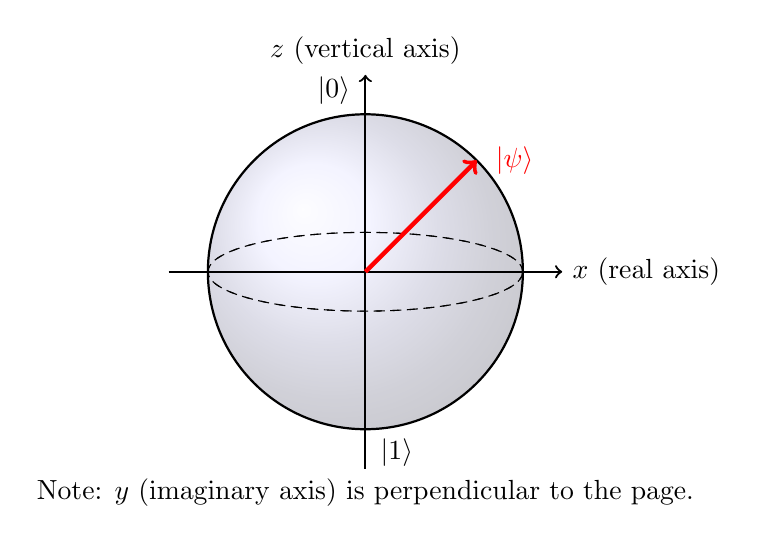
\begin{tikzpicture}[scale=1]
    % Draw sphere outline with shading
    \shade[ball color=blue!20, opacity=0.3] (0,0) circle (2cm);
    \draw[thick] (0,0) circle (2cm);
    
    % Draw equator as a dashed ellipse (horizontal cross-section)
    \draw[dashed] (0,0) ellipse (2cm and 0.5cm);
    
    % Draw meridian arcs (vertical cross-sections)
    \draw[dashed] (-2,0) arc (180:0:2cm and 0.5cm);
    \draw[dashed] (2,0) arc (0:-180:2cm and 0.5cm);
    
    % Axes: x and z
    \draw[->, thick] (-2.5,0) -- (2.5,0) node[right] {$x$ (real axis)};
    \draw[->, thick] (0,-2.5) -- (0,2.5) node[above] {$z$ (vertical axis)};
    
    % Mark north and south poles with horizontal shift
    \node[above, xshift=-0.4cm] at (0,2) {\(|0\rangle\)};
    \node[below, xshift=0.4cm] at (0,-2) {\(|1\rangle\)};
    
    % Bloch vector in the x-z plane
    \draw[->, red, ultra thick] (0,0) -- (1.414,1.414) node[right] {\(\;|\psi\rangle\)};
    
    % Note for y axis
    \node at (0,-2.8) {Note: \(y\) (imaginary axis) is perpendicular to the page.};
  \end{tikzpicture}
  \caption{Enhanced Bloch sphere representation of a \gls{qubit} with adjusted labels.}
  \label{fig:bloch_sphere}
  \end{figure}

\begin{observation}
  For multi-qubit systems, the overall state space is given by the tensor product of individual qubit spaces. For instance, a two-qubit system is described by
  \[
  |\psi\rangle = \sum_{i,j \in \{0,1\}} \alpha_{ij}\, |i\rangle \otimes |j\rangle, \quad \sum_{i,j} |\alpha_{ij}|^2 = 1.
  \]
  This exponential scaling of the state space underpins the potential of quantum parallelism \cite{nielsen2010quantum}.
\end{observation}



\subsection{Superposition and Entanglement}
\label{subsec:superposition}

\textbf{Superposition} enables parallel computation. The Hadamard gate ($H$) creates uniform superpositions:
\[
H|0\rangle = \frac{|0\rangle + |1\rangle}{\sqrt{2}}, \quad H|1\rangle = \frac{|0\rangle - |1\rangle}{\sqrt{2}}.
\]

\textbf{Entanglement} arises in multi-qubit states that cannot be factored. The Bell states are maximally entangled:
\[
|\Phi^+\rangle = \frac{|00\rangle + |11\rangle}{\sqrt{2}}, \quad |\Phi^-\rangle = \frac{|00\rangle - |11\rangle}{\sqrt{2}},
\]
\[
|\Psi^+\rangle = \frac{|01\rangle + |10\rangle}{\sqrt{2}}, \quad |\Psi^-\rangle = \frac{|01\rangle - |10\rangle}{\sqrt{2}}.
\]

\begin{figure}[h]
\centering
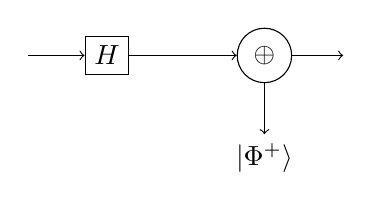
\begin{tikzpicture}
  \node[draw,rectangle] (h) at (0,0) {$H$};
  \node[draw,circle] (cnot) at (2,0) {$\oplus$};
  \draw[->] (-1,0) -- (h);
  \draw[->] (h) -- (cnot);
  \draw[->] (cnot) -- (3,0);
  \draw[->] (cnot) -- (2,-1) node[below] {$|\Phi^+\rangle$};
\end{tikzpicture}
\caption{Quantum circuit generating the Bell state $|\Phi^+\rangle$.}
\label{fig:bell_circuit}
\end{figure}

Entanglement is critical for quantum teleportation \cite{bennett1993teleporting} and enables exponential speedups in algorithms like Shor's \cite{shor1999polynomial}.

\subsection{Quantum Gates and Circuits}
\label{subsec:gates}

Quantum gates are the building blocks of quantum circuits. They are represented by \emph{unitary operators} \(U\) (i.e. \(U^\dagger U = I\)) that govern the evolution of quantum states. Key single-qubit gates include:
\begin{itemize}
    \item \textbf{Pauli-X (bit-flip):} 
    \[
    X = \begin{pmatrix} 0 & 1 \\ 1 & 0 \end{pmatrix},
    \]
    which acts as \(X|0\rangle = |1\rangle\) and \(X|1\rangle = |0\rangle\).
    \item \textbf{Hadamard (creating superpositions):}
    \[
    H = \frac{1}{\sqrt{2}}\begin{pmatrix} 1 & 1 \\ 1 & -1 \end{pmatrix}.
    \]
    \item \textbf{Phase shift:}
    \[
    R_\phi = \begin{pmatrix} 1 & 0 \\ 0 & e^{i\phi} \end{pmatrix}.
    \]
\end{itemize}

Two-qubit gates, such as the \textbf{Controlled-NOT (CNOT) gate}, introduce entanglement. The CNOT gate acts on a pair of qubits as
\[
\text{CNOT}|a\rangle|b\rangle = |a\rangle|a \oplus b\rangle,
\]
where \(\oplus\) denotes addition modulo 2.

Quantum circuits decompose complex algorithms into sequences of gate operations. A universal gate set (e.g., \(\{H, T, \text{CNOT}\}\)) can approximate any unitary operation to arbitrary precision, forming the basis for the quantum circuit model.

Figure~\ref{fig:deutsch_circuit} shows an example quantum circuit used in the Deutsch-Jozsa algorithm, illustrating the interplay of Hadamard gates and entangling operations.

\begin{figure}[h]
\centering
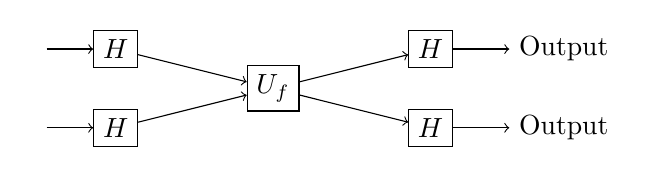
\begin{tikzpicture}[node distance=1.8cm, auto]
    \node (in1) at (0,0) {};
    \node (in2) at (0,-1) {};
    \node[draw, rectangle] (H1) at (1,0) {$H$};
    \node[draw, rectangle] (H2) at (1,-1) {$H$};
    \node[draw, rectangle] (Uf) at (3, -0.5) {\(U_f\)};
    \node[draw, rectangle] (H3) at (5,0) {$H$};
    \node[draw, rectangle] (H4) at (5,-1) {$H$};
    \draw[->] (in1) -- (H1);
    \draw[->] (in2) -- (H2);
    \draw[->] (H1) -- (Uf);
    \draw[->] (H2) -- (Uf);
    \draw[->] (Uf) -- (H3);
    \draw[->] (Uf) -- (H4);
    \draw[->] (H3) -- ++(1,0) node[right] {Output};
    \draw[->] (H4) -- ++(1,0) node[right] {Output};
\end{tikzpicture}
\caption{Quantum circuit for the Deutsch-Jozsa algorithm.}
\label{fig:deutsch_circuit}
\end{figure}

\subsection{Measurement and Probabilistic Outcomes}
\label{subsec:measurement}

Measurement collapses a state to a basis vector. For $|\psi\rangle = \sum_i \alpha_i|i\rangle$, the probability of outcome $i$ is $|\alpha_i|^2$ (Born rule). For example, measuring $|\Phi^+\rangle$ in the computational basis yields $|00\rangle$ or $|11\rangle$ with 50\% probability each.

\begin{table}[h]
\centering
\caption{Measurement outcomes for $|\Phi^+\rangle$.}
\label{tab:bell_measurement}
\begin{tabular}{|c|c|}
\hline
\textbf{Outcome} & \textbf{Probability} \\ \hline
$|00\rangle$      & 50\%                \\ \hline
$|11\rangle$      & 50\%                \\ \hline
\end{tabular}
\end{table}

Mixed states are described by density matrices $\rho = \sum_i p_i |\psi_i\rangle\langle\psi_i|$. This formalism is essential for open quantum systems \cite{breuer2002theory}.
\subsection{Decoherence and Open Systems}
\label{subsec:decoherence}

Decoherence arises from environment interactions, modeled by the Lindblad equation:
\[
\frac{d\rho}{dt} = -\frac{i}{\hbar}[H, \rho] + \sum_k \left( L_k \rho L_k^\dagger - \frac{1}{2}\{L_k^\dagger L_k, \rho\} \right),
\]
where $L_k$ are Lindblad operators \cite{breuer2002theory}. Common noise models include:
- \textbf{Amplitude damping}: Energy loss to the environment.
- \textbf{Phase damping}: Loss of phase coherence.

\begin{figure}[h]
\centering
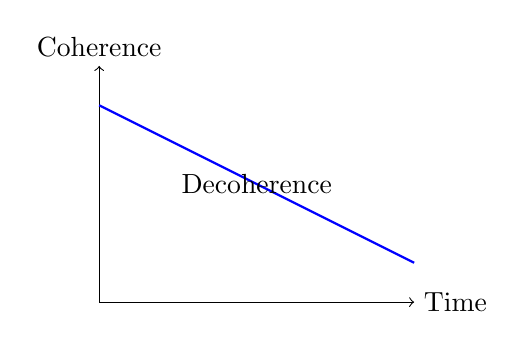
\begin{tikzpicture}
  \draw[->] (0,0) -- (4,0) node[right] {Time};
  \draw[->] (0,0) -- (0,3) node[above] {Coherence};
  \draw[thick,blue] (0,2.5) -- (4,0.5);
  \node at (2,1.5) {Decoherence};
\end{tikzpicture}
\caption{Decoherence reduces quantum state fidelity over time.}
\label{fig:decoherence}
\end{figure}

Quantum error correction codes, like the Shor code \cite{shor1995scheme}, mitigate decoherence by encoding logical qubits into multiple physical qubits. 

\subsection{Additional Remarks: Unitary Evolution and Quantum Dynamics}
\label{subsec:unitary_evolution}

\begin{definition}[Unitary Evolution]
In a closed quantum system, the state evolution is governed by the Schrödinger equation,
\[
i\hbar \frac{d}{dt} |\psi(t)\rangle = H |\psi(t)\rangle,
\]
where \(H\) is the Hamiltonian. The solution to this equation is given by
\[
|\psi(t)\rangle = U(t)|\psi(0)\rangle, \quad \text{with } U(t)=e^{-iHt/\hbar},
\]
where \(U(t)\) is a unitary operator.
\end{definition}

\begin{remark}
Unitary evolution is reversible and forms the basis for the operation of quantum circuits, where continuous evolution is discretized into sequences of quantum gates.
\end{remark}

\begin{theorem}[No-Cloning Theorem]
    Let \(\mathcal{H}\) be a Hilbert space with \(\dim \mathcal{H} \ge 2\). There is no unitary operator \(U\) such that for all states \(|\psi\rangle \in \mathcal{H}\) the following holds:
    \[
    U\big(|\psi\rangle \otimes |0\rangle\big) = |\psi\rangle \otimes |\psi\rangle.
    \]
\end{theorem}

\begin{observation}
    The \textbf{no-cloning theorem} states that it is impossible to create an exact copy of an arbitrary unknown quantum state. This fundamental principle has significant implications for quantum information processing and quantum cryptography.
    The no-cloning theorem ensures that quantum information cannot be perfectly replicated, which underpins the security of many quantum cryptographic protocols.
\end{observation}    